\documentclass[9pt]{article}
\usepackage[utf8]{inputenc}
\usepackage{amsmath,amsthm,amsfonts,amssymb,amscd}
\usepackage{multirow,booktabs}
\usepackage{enumitem}
\usepackage{fancyhdr}
\usepackage{mathrsfs}
\usepackage{wrapfig}
\usepackage{setspace}
\usepackage{calc}
\usepackage{multicol}
\usepackage{cancel}
\usepackage[retainorgcmds]{IEEEtrantools}
\usepackage{framed}
\usepackage[most]{tcolorbox}
\usepackage{tikz}
\usepackage{geometry}
\geometry{
	a4paper,
	total={170mm,257mm},
	left=20mm,
	top=20mm,
}
\title{Further on Magnetic Fields \& Forces}
\author{Aaron G.K.}
\begin{document}
	\maketitle
		\section*{Motor Effect}
		We have seen that a current carrying wire experiences a force when it is inserted into an external magnetic field. However, what if it was a loop of wire instead of being a straight wire? We will see that it will have a turning effect and that effect is used in almost every motor technology. For example, let's talk a look at the wire loop in the uniform magnetic field below.
		\begin{center}
			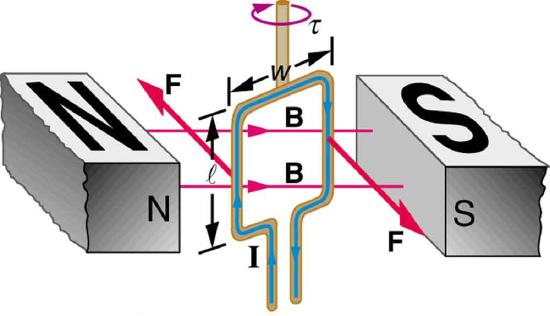
\includegraphics[scale=0.4]{torque_current_loop.jpg}
		\end{center}
		We can deduce the force in each segment of the loop as follows \begin{enumerate}
			\item For the left segment, the current is going upwards: thus, we say the direction of the vector $\vec{l}$ is $\hat{j}$. Since we know the magnetic field is directed to the right through out the whole:
			$$\vec{F}=I\vec{l}\times\vec{B}$$
			$$\vec{F}=\hat{j}\times\hat{i}$$
			$$\vec{F}=-\hat{k}$$
			The magnitude of the force on the first segment is $F=IlB\sin\theta=IlB$ 
			\item For the top segment, the current is going to the right: thus, we say the direction of the vector $\vec{l}$ is $\hat{i}$. Since we know the magnetic field is directed to the right through out the whole:
			$$\vec{F}=I\vec{l}\times\vec{B}$$
			$$\vec{F}=\hat{i}\times\hat{i}$$
			$$\vec{F}=0$$
			The magnitude of the force on the first segment is $F=IlB\sin\theta=0$ since $\vec{l}\parallel vec{B}$
			\item For the right segment, the current is going downwards: thus, we say the direction of the vector $\vec{l}$ is -$\hat{j}$. Since we know the magnetic field is directed to the right through out the whole:
			$$\vec{F}=I\vec{l}\times\vec{B}$$
			$$\vec{F}=-\hat{j}\times\hat{i}$$
			$$\vec{F}=\hat{k}$$
			The magnitude of the force on the first segment is $F=IlB\sin\theta=IlB$ 
			\item For the bottom segment, the current is going to the left: thus, we say the direction of the vector $\vec{l}$ is $\hat{i}$. Since we know the magnetic field is directed to the right through out the whole:
			$$\vec{F}=I\vec{l}\times\vec{B}$$
			$$\vec{F}=-\hat{i}\times\hat{i}$$
			$$\vec{F}=0$$
			The magnitude of the force on the first segment is $F=IlB\sin\theta=0$ since $\vec{l}\parallel vec{B}$
		\end{enumerate}
		From the above computations, we can see that the there is no forces on the bottom and top segments of the wire when the wire is sitting on the plane of the page. However, on the left and right segments. Specifically, the force on the left segment is acting into the page while the force on the right segment is acting out of the page. The combination of the forces here creates a turning effect. We can quantify the torque on the left and right segment as follows:
		
		\begin{enumerate}
			\item $$\tau_{left}=r_1F_1\sin\theta$$
			We can see that $r_1$ is the distance between where $F_1$ is acting and the axis of rotation of the loop. We can see that the axis of rotation is on the vertical line cutting the loop into two halves. Thus, $r_1=r_3=\dfrac{w}{2}$
			$$\tau_{left}=\dfrac{w}{2}(IlB)\sin\theta$$
			\item $$\tau_{right}=r_3F_3\sin\theta$$
			We can see that $r_3$ is the distance between where $F_3$ is acting and the axis of rotation of the loop. We have seen above that $r_1=r_3=\dfrac{w}{2}$
			$$\tau_{right}=\dfrac{w}{2}(IlB)\sin\theta$$
		\end{enumerate}
		We can see, however, that the torques turn in the same direction. Thus, we add the two torques to get the total torque on the loop.
		$$\tau=\tau_{left}+\tau_{right}$$
		$$\tau=\dfrac{w}{2}(IlB)\sin\theta+\dfrac{w}{2}(IlB)\sin\theta$$
		$$\tau=(wIlB)\sin\theta\implies(wlIB)\sin\theta$$
		$$\tau=(AIB)\sin\theta\text{ since } wl=A$$
		In real life applications of the motor effect, it is rare to use just a single loop because the torque we would get is not much. Thus, we use multiple(usually hundreds) loops that are identical. Since the current is the same in each loop and they all roughly have the same area, the total torque is the number of the loops multiplied by the torque produced by a single loop.
		$$\tau=NAIB\sin\theta$$ 
		\subsection*{Magnetic Fields of Different Structures}
		\subsubsection*{Magnetic Field of a Solenoid}
		A long wire wound in the form of a helical coil is known as a solenoid. Solenoids are commonly used in experimental research requiring magnetic fields. What makes a solenoid special is that it is generally easy to wind, and near its center, its magnetic field is quite uniform and directly proportional to the current in the wire.
		\begin{center}
			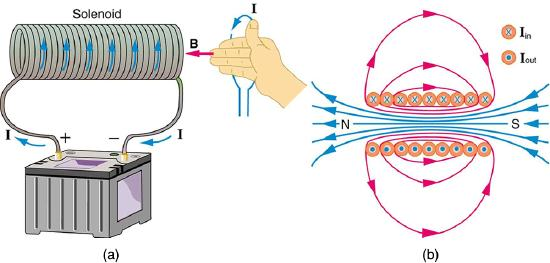
\includegraphics[scale=0.5]{solenoid}
		\end{center}
		From the figure above, we can see that a solenoid has a magnetic field very similar to a bar magnet and hence, it behaves as one. Solenoids are very valuable because we can output the exact amount of magnetic field we want by changing the current through the solenoid. The magnetic field strength at the center of a solenoid is affected by many factors including the number of coils per unit length and the current through the coil. It is mathematically given as:
		$$B=\mu_onI\text{ where }n\text{is the number of coils per unit length }\&\text{ }n=\dfrac{N}{L}$$
		Similarly we can express this in terms of the number of loops and the total length of the coil:
		$$B=\mu_o\dfrac{N}{L}I$$
		\subsubsection*{Magnetic Field of a Toroid}
		\begin{center}
			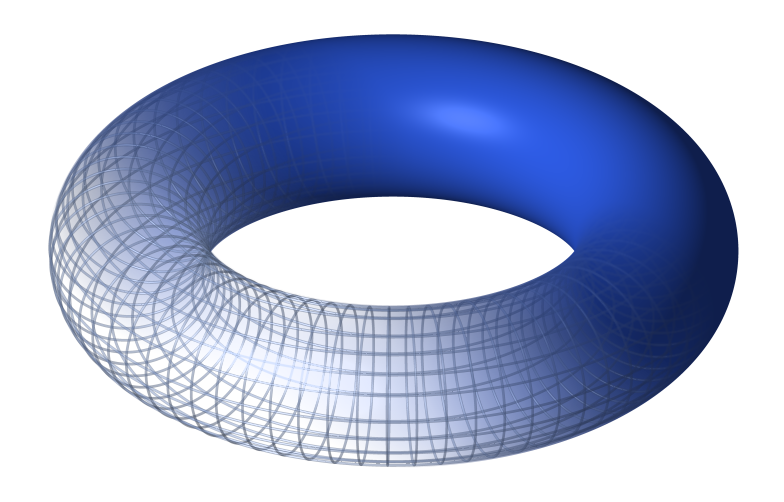
\includegraphics[scale=0.3]{toroid}
		\end{center}	
		You can think of a toroid as a solenoid that has been bent into the shape of a circle (a torus, actually), as illustrated above.
		Inside the toroid, the magnetic field forms concentric circles as shown below:
		\begin{center}
			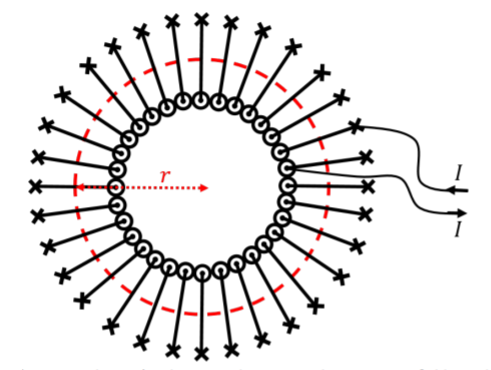
\includegraphics[scale=0.3]{torus_field}
		\end{center}
		Similar to a solenoid, the magnetic field of a toroid is affected by the current through the coils and the number of coils in total.
		$$B=\frac{\mu_{0}NI}{2\pi r} $$
		\subsubsection*{ADVANCED: Ampere's Law}
		Generally, for different coils having various geometrical shapes of wire, we use Ampere's law to calculate the magnetic field generated by the current carrying wire. Ampere's Law states that for an arbitrary closed path in which current is flowing, the magnetic field is given by:
		$$\oint \vec{B} \cdot d\vec{l} = \mu_0 I_{enc}$$
		where I is the total current passing through any open surface S whose perimeter is the path of integration. 
		
		
\end{document}	